\documentclass[9pt,a4paper]{article}

\usepackage[a4paper,margin=0.55in]{geometry}
\usepackage{amsmath,amssymb}
\usepackage{booktabs,array}
\usepackage{tikz}
\usepackage{pgfplots}
\usepackage{xcolor}
\usepackage{microtype}
\usepackage{enumitem}
\usepackage{tcolorbox}
\usepackage{multicol}
\usepackage{fancyhdr}
\usepackage[hidelinks]{hyperref}
\usepackage{lmodern}
\usetikzlibrary{arrows.meta,positioning,fit,calc}
\pgfplotsset{compat=1.18}

\setlength{\parindent}{0pt}
\setlength{\parskip}{2.0pt}
\setlist{nosep,leftmargin=1.25em}
\renewcommand{\arraystretch}{1.0}
\urlstyle{same}

\definecolor{SGDark}{HTML}{123F39}
\definecolor{SGGreen}{HTML}{2E755B}
\definecolor{SGLight}{HTML}{A9D19E}
\definecolor{SGMint}{HTML}{E6EEDD}
\definecolor{SGCream}{HTML}{F5F1E3}
\definecolor{SGGold}{HTML}{CDA344}
\definecolor{SGText}{HTML}{1D3531}
\definecolor{SGGray}{HTML}{66716D}
\definecolor{SGLine}{HTML}{C7C3B1}

\newcommand{\HL}{\ensuremath{H_L}}
\newcommand{\SL}{\ensuremath{S_L}}
\newcommand{\LER}{\ensuremath{\mathrm{LER}}}
\newcommand{\Utility}{\ensuremath{\mathrm{Utility}}}
\newcommand{\pp}{\ensuremath{\mathrm{pp}}}

\newtcolorbox{boxg}[1][]{colback=SGCream,colframe=SGLine,boxrule=.55pt,arc=3pt,left=6pt,right=6pt,top=4pt,bottom=4pt,#1}
\newtcolorbox{boxm}[1][]{colback=SGMint,colframe=SGGreen,boxrule=.65pt,arc=3pt,left=6pt,right=6pt,top=4pt,bottom=4pt,#1}

\pagestyle{fancy}
\fancyhf{}
\lhead{\textcolor{SGDark}{\textbf{SecureGate}}}
\rhead{\textcolor{SGGray}{Public Technical Report • 2026}}
\cfoot{\textcolor{SGGray}{\thepage}}
\renewcommand{\headrulewidth}{0.3pt}
\renewcommand{\footrulewidth}{0pt}

\pgfplotsset{
 every axis/.append style={
  font=\scriptsize,
  tick label style={font=\scriptsize},
  label style={font=\scriptsize},
  title style={font=\small\bfseries,text=SGDark},
  axis line style={draw=SGDark!75},
  tick style={draw=SGDark!75},
  grid=major,
  major grid style={draw=SGLine!40},
  xmajorgrids=false,
  ymajorgrids=true,
 }
}

\begin{document}

\begin{center}
{\color{SGDark}\bfseries\Large SecureGate: Mitigating Gate-Fingerprint Leakage in Fault-Tolerant Quantum Computing}\par
\vspace{2pt}
{\large\bfseries Marya Alturki}\par
\vspace{2pt}
{\small Circuit-level proof of concept for randomized virtual Pauli-error mitigation}
\end{center}

\begin{boxg}
\textbf{Abstract.} SecureGate is a proof-of-concept security approach for fault-tolerant quantum computing that addresses decoder-side gate-fingerprint leakage. We study whether an untrusted decoder can infer hidden logical operations from spacetime syndrome data and evaluate randomized circuit-level virtual Pauli errors as a mitigation. In distance-5 surface-code simulations, mitigation reduced gate-inference accuracy from 53.81\% to 53.41\% while maintaining approximately 99.42\% decoder utility.
\end{boxg}

\section*{1. Problem and Research Question}
Fault-tolerant quantum computers repeatedly extract syndrome information and pass detector records to a classical decoder. Recent research identifies a confidentiality threat in which gate-dependent statistical structure in spacetime syndrome data can expose information about a hidden logical operation to an untrusted decoder \cite{shukla2026}.

\begin{boxm}\centering\textbf{Research question:} Can randomized virtual Pauli errors introduced at the circuit level perturb gate-dependent detector information while preserving measured decoder performance?\end{boxm}

\section*{2. SecureGate Mind Map}
\begin{center}
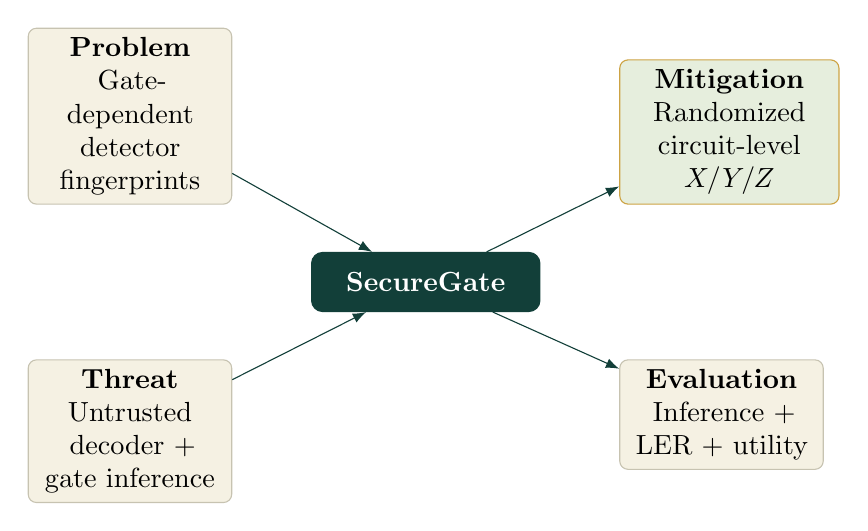
\begin{tikzpicture}[node distance=6mm and 10mm,>=Latex]
\node[draw=SGDark,fill=SGDark,text=white,rounded corners=4pt,minimum width=2.9cm,minimum height=.75cm,align=center,font=\bfseries] (c) {SecureGate};
\node[draw=SGLine,fill=SGCream,rounded corners=3pt,align=center,text width=2.35cm,above left=of c] (p) {\textbf{Problem}\\Gate-dependent detector fingerprints};
\node[draw=SGLine,fill=SGCream,rounded corners=3pt,align=center,text width=2.35cm,below left=of c] (a) {\textbf{Threat}\\Untrusted decoder + gate inference};
\node[draw=SGGold,fill=SGMint,rounded corners=3pt,align=center,text width=2.55cm,above right=of c] (m) {\textbf{Mitigation}\\Randomized circuit-level $X/Y/Z$};
\node[draw=SGLine,fill=SGCream,rounded corners=3pt,align=center,text width=2.35cm,below right=of c] (e) {\textbf{Evaluation}\\Inference + $\LER$ + utility};
\draw[-Latex,SGDark] (p) -- (c);
\draw[-Latex,SGDark] (a) -- (c);
\draw[-Latex,SGDark] (c) -- (m);
\draw[-Latex,SGDark] (c) -- (e);
\end{tikzpicture}
\end{center}

\section*{3. What Is New in SecureGate?}
SecureGate connects gate-fingerprint measurement to an explicit circuit-level mitigation experiment. Rather than modifying detector records after measurement, the final experiment inserts a perfect Pauli instruction into the fault-tolerant circuit, propagates the Pauli frame, and directly resamples the altered circuit. The decoder used for evaluation is left unchanged. The Pauli-frame component follows the established principle of classical Pauli tracking through Clifford circuits \cite{reichardt2006}.

\begin{boxg}
\textbf{Scientific scope.} Gate-inference accuracy is an empirical measure of the performance of the specified Bernoulli Naive Bayes inference model. It is not a percentage of information leakage and does not quantify optimal adversarial inference.
\end{boxg}

\section*{4. Main Experiment at a Glance}
\begin{center}
\begin{tabular}{>{\bfseries}p{0.28\linewidth} p{0.63\linewidth}}
\toprule
Code / circuit & Unrotated CSS surface code, distance 5\\
Physical resources & 81 physical qubits = 41 data + 40 ancilla\\
Logical operations & \HL{} and \SL{}; 100 detectors; 1 logical observable each\\
Noise parameter & $p=10^{-3}$\\
Sampling & 10,000 shots per gate per run\\
Repeated evaluation & 10 independent baseline runs + 10 mitigation runs\\
Mitigation space & 41 data qubits $\times$ $\{X,Y,Z\}$ = 123 cases\\
Inference / decoder & Bernoulli Naive Bayes / matching decoder on \SL{}\\
\bottomrule
\end{tabular}
\end{center}

\section*{5. Methodology}
\begin{center}
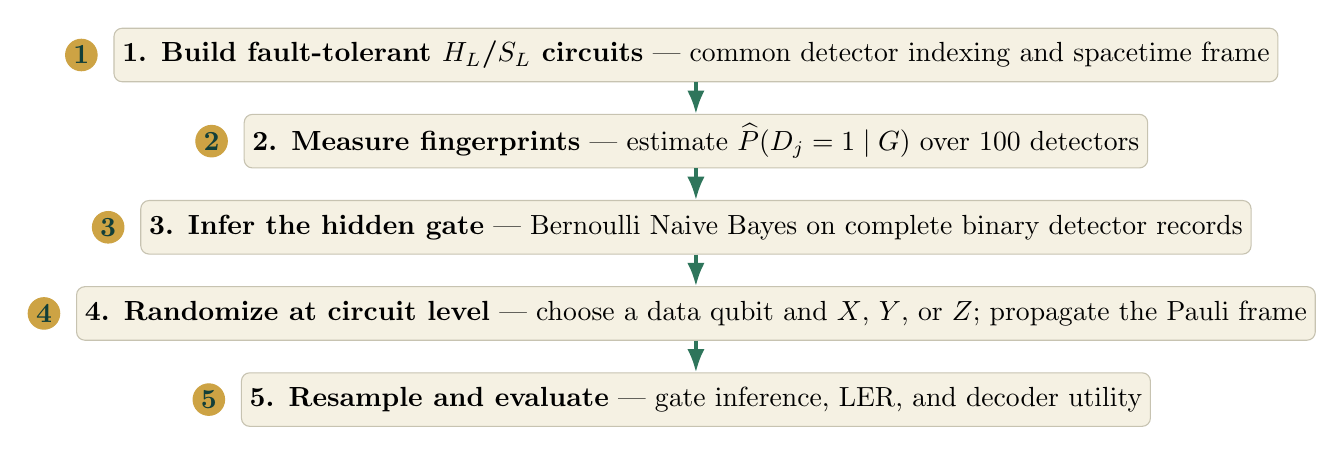
\begin{tikzpicture}[node distance=4mm,>=Latex]
\tikzset{mstep/.style={draw=SGLine,fill=SGCream,rounded corners=3pt,minimum width=.90\linewidth,minimum height=.68cm,align=center,inner sep=3pt},mnum/.style={circle,draw=SGGold,fill=SGGold,text=SGDark,font=\bfseries,minimum size=.4cm,inner sep=0pt}}
\node[mstep] (s1) {\textbf{1. Build fault-tolerant \HL/\SL{} circuits} — common detector indexing and spacetime frame};\node[mnum,left=2mm of s1.west] {1};
\node[mstep,below=of s1] (s2) {\textbf{2. Measure fingerprints} — estimate $\widehat P(D_j=1\mid G)$ over 100 detectors};\node[mnum,left=2mm of s2.west] {2};
\node[mstep,below=of s2] (s3) {\textbf{3. Infer the hidden gate} — Bernoulli Naive Bayes on complete binary detector records};\node[mnum,left=2mm of s3.west] {3};
\node[mstep,below=of s3] (s4) {\textbf{4. Randomize at circuit level} — choose a data qubit and $X$, $Y$, or $Z$; propagate the Pauli frame};\node[mnum,left=2mm of s4.west] {4};
\node[mstep,below=of s4] (s5) {\textbf{5. Resample and evaluate} — gate inference, $\LER$, and decoder utility};\node[mnum,left=2mm of s5.west] {5};
\draw[-Latex,very thick,SGGreen] (s1) -- (s2);
\draw[-Latex,very thick,SGGreen] (s2) -- (s3);
\draw[-Latex,very thick,SGGreen] (s3) -- (s4);
\draw[-Latex,very thick,SGGreen] (s4) -- (s5);
\end{tikzpicture}
\end{center}

\subsection*{5.1 Detector Fingerprints}
For detector $j$ and logical gate $G$, the empirical event probability is
\[
\widehat P(D_j=1\mid G)=\frac{1}{N}\sum_{k=1}^{N}D_j^{(k)},\qquad N=10{,}000.
\]
Notebook 03 found mean detector-event probabilities of 0.024598 for \HL{} and 0.026675 for \SL{}. The mean absolute detector-wise difference was 0.003681, with a maximum of 0.019200 at detector 52 and $t=1.0$. The full 100-detector profiles remained highly correlated ($r=0.950529$) while retaining nonzero detector-level structure.

\subsection*{5.2 Gate Inference}
A balanced dataset of 20,000 records (10,000 per gate) was evaluated with an 80/20 stratified split using Bernoulli Naive Bayes. The seed-42 test split gave 55.27\% accuracy (95\% Wilson interval [53.73\%, 56.81\%]). Repeated split, fresh-shot, and label-permutation controls supported a measurable but modest gate-dependent signal; the permutation control was 50.02\%.

\subsection*{5.3 Circuit-Level Virtual Pauli Mitigation}
The mitigation library contains all $41\times3=123$ data-qubit/Pauli cases. A virtual error is selected independently for each shot with probability $\alpha=0.50$, with the data qubit and Pauli type sampled uniformly from the library. The same rule is used for \HL{} and \SL{} and does not depend on the hidden gate label.

A Pauli frame is represented by $I=(0,0)$, $X=(1,0)$, $Y=(1,1)$, and $Z=(0,1)$. For the relevant Clifford operations,
\[
H:(x,z)\mapsto(z,x),\qquad S:(x,z)\mapsto(x,z\oplus x),
\]
with the corresponding controlled-$Z$ and SWAP propagation rules. This follows the classical Pauli-tracking principle \cite{reichardt2006}.

\subsection*{5.4 Evaluation}
Gate-inference accuracy is the fraction of correctly classified test records. For the \SL{} decoder evaluation,
\[
\LER=\frac{N_{\mathrm{logical\ errors}}}{N_{\mathrm{shots}}},\qquad \Utility=1-\LER.
\]
The final comparison uses ten independent runs per condition with fresh circuit sampling and new virtual-error realizations in the mitigation runs.

\clearpage
\section*{6. Results}
\begin{center}
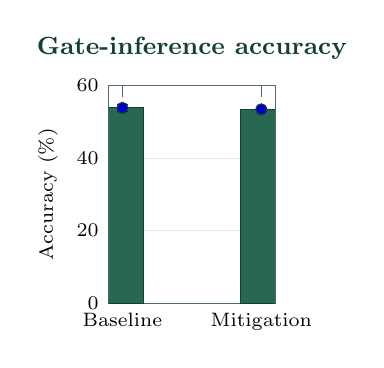
\begin{tikzpicture}
\begin{axis}[title={Gate-inference accuracy},ylabel={Accuracy (\%)},ymin=0,ymax=60,xtick=data,xticklabels={Baseline,Mitigation},width=.305\linewidth,height=4.35cm,bar width=15pt]
\addplot+[ybar,fill=SGGreen!88!black,draw=SGDark,error bars/.cd,y dir=both,y explicit] coordinates {(0,53.810)+-(0,0.950) (1,53.408)+-(0,0.629)};
\end{axis}
\end{tikzpicture}\hspace{1mm}
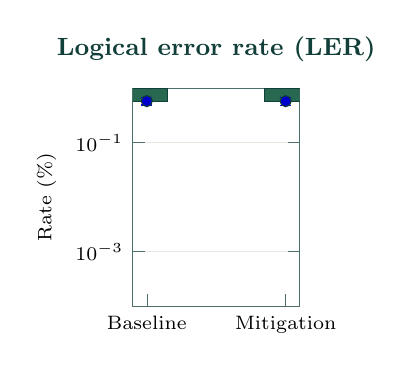
\begin{tikzpicture}
\begin{axis}[title={Logical error rate (LER)},ylabel={Rate (\%)},ymode=log,ymin=0.0001,ymax=1,xtick=data,xticklabels={Baseline,Mitigation},width=.305\linewidth,height=4.35cm,bar width=15pt]
\addplot+[ybar,fill=SGGreen!88!black,draw=SGDark,error bars/.cd,y dir=both,y explicit] coordinates {(0,0.579)+-(0,0.087) (1,0.577)+-(0,0.104)};
\end{axis}
\end{tikzpicture}\hspace{1mm}
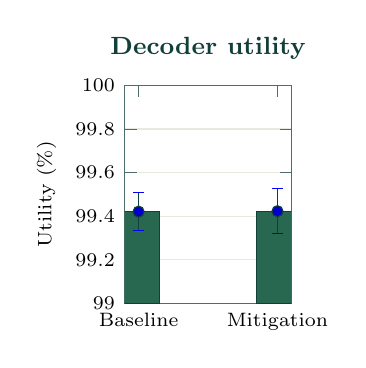
\begin{tikzpicture}
\begin{axis}[title={Decoder utility},ylabel={Utility (\%)},ymin=99.0,ymax=100.0,xtick=data,xticklabels={Baseline,Mitigation},width=.305\linewidth,height=4.35cm,bar width=15pt]
\addplot+[ybar,fill=SGGreen!88!black,draw=SGDark,error bars/.cd,y dir=both,y explicit] coordinates {(0,99.421)+-(0,0.087) (1,99.423)+-(0,0.104)};
\end{axis}
\end{tikzpicture}
\end{center}

\begin{center}
\begin{tabular}{lccc}
\toprule
\textbf{Metric} & \textbf{Baseline} & \textbf{Mitigation} & \textbf{Change}\\
\midrule
Gate inference & 53.810\% $\pm$ 0.950\,\pp & 53.408\% $\pm$ 0.629\,\pp & $-0.403$\,\pp\\
\LER & 0.579\% $\pm$ 0.087\,\pp & 0.577\% $\pm$ 0.104\,\pp & $-0.002$\,\pp\\
Decoder utility & 99.421\% $\pm$ 0.087\,\pp & 99.423\% $\pm$ 0.104\,\pp & $+0.002$\,\pp\\
\bottomrule
\end{tabular}
\end{center}

\begin{center}
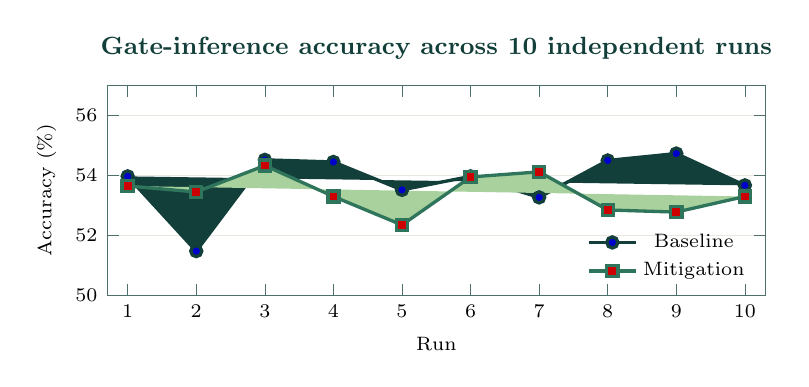
\begin{tikzpicture}
\begin{axis}[title={Gate-inference accuracy across 10 independent runs},xlabel={Run},ylabel={Accuracy (\%)},xmin=.7,xmax=10.3,ymin=50,ymax=57,xtick={1,...,10},legend style={at={(0.99,0.02)},anchor=south east,draw=none,fill=none,font=\scriptsize},width=.82\linewidth,height=4.25cm]
\addplot+[very thick,mark=*,draw=SGDark,fill=SGDark] coordinates {(1,53.97)(2,51.48)(3,54.52)(4,54.45)(5,53.52)(6,53.97)(7,53.27)(8,54.50)(9,54.73)(10,53.67)};\addlegendentry{Baseline}
\addplot+[very thick,mark=square*,draw=SGGreen,fill=SGLight] coordinates {(1,53.65)(2,53.45)(3,54.33)(4,53.30)(5,52.35)(6,53.95)(7,54.12)(8,52.85)(9,52.78)(10,53.30)};\addlegendentry{Mitigation}
\end{axis}
\end{tikzpicture}
\end{center}

\begin{boxm}
\textbf{Main finding.} Across ten independent runs, gate-inference accuracy changed from 53.810\% to 53.408\% (about $-0.403$ percentage points), while \LER and decoder utility remained essentially unchanged. The observed reduction is small and is not treated as statistically conclusive.
\end{boxm}

\section*{7. Interpretation}
\begin{multicols}{2}
\textbf{Leakage indicator.} The baseline experiment shows a measurable, reproducible gate-dependent signal in the simulated \HL/\SL{} detector records, but the classifier is deliberately treated as a baseline inference model rather than an optimal adversary.

\textbf{Mitigation effect.} The circuit-level virtual-Pauli experiment is associated with a small decrease in measured inference accuracy. The magnitude is modest relative to run-to-run variability, so stronger claims require broader testing.

\columnbreak

\textbf{Decoder performance.} The measured \LER changes by $-0.002\pp$ and utility by $+0.002\pp$. In the tested setting, the mitigation therefore did not materially change the measured decoder performance.

\textbf{What the result does not show.} It does not establish elimination of leakage, a universal privacy guarantee, optimal attack resistance, or general hardware-level security.
\end{multicols}

\clearpage
\section*{8. Limitations and Future Work}
\begin{center}
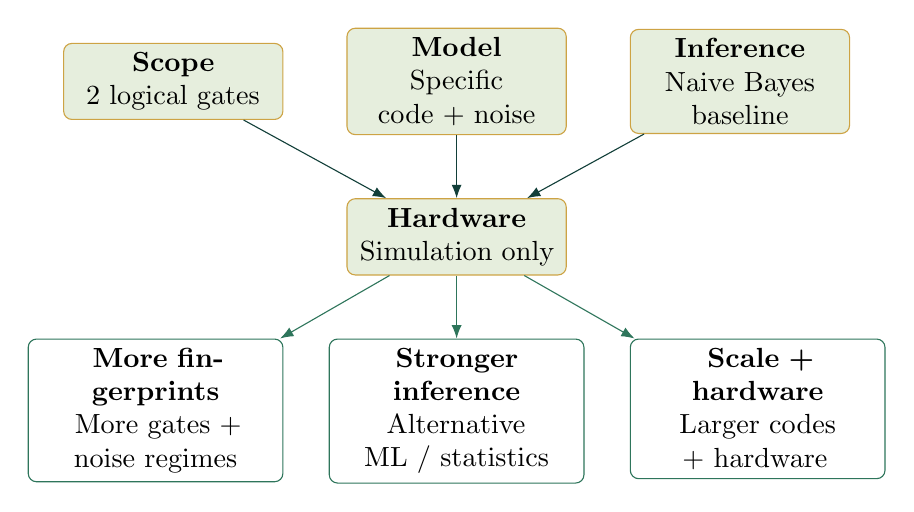
\begin{tikzpicture}[node distance=8mm and 8mm,>=Latex]
\node[draw=SGGold,fill=SGMint,rounded corners=3pt,text width=2.55cm,minimum height=.9cm,align=center] (l1) {\textbf{Scope}\\2 logical gates};
\node[draw=SGGold,fill=SGMint,rounded corners=3pt,text width=2.55cm,minimum height=.9cm,align=center,right=of l1] (l2) {\textbf{Model}\\Specific code + noise};
\node[draw=SGGold,fill=SGMint,rounded corners=3pt,text width=2.55cm,minimum height=.9cm,align=center,right=of l2] (l3) {\textbf{Inference}\\Naive Bayes baseline};
\node[draw=SGGold,fill=SGMint,rounded corners=3pt,text width=2.55cm,minimum height=.9cm,align=center,below=of l2] (l4) {\textbf{Hardware}\\Simulation only};
\node[draw=SGGreen,fill=white,rounded corners=3pt,text width=3.0cm,minimum height=.9cm,align=center,below left=of l4] (n1) {\textbf{More fingerprints}\\More gates + noise regimes};
\node[draw=SGGreen,fill=white,rounded corners=3pt,text width=3.0cm,minimum height=.9cm,align=center,below=of l4] (n2) {\textbf{Stronger inference}\\Alternative ML / statistics};
\node[draw=SGGreen,fill=white,rounded corners=3pt,text width=3.0cm,minimum height=.9cm,align=center,below right=of l4] (n3) {\textbf{Scale + hardware}\\Larger codes + hardware};
\draw[-Latex,SGDark] (l1) -- (l4);
\draw[-Latex,SGDark] (l2) -- (l4);
\draw[-Latex,SGDark] (l3) -- (l4);
\draw[-Latex,SGGreen] (l4) -- (n1);
\draw[-Latex,SGGreen] (l4) -- (n2);
\draw[-Latex,SGGreen] (l4) -- (n3);
\end{tikzpicture}
\end{center}

\section*{9. Conclusion}
SecureGate demonstrates a circuit-level proof of concept for evaluating randomized virtual Pauli errors as a mitigation strategy against decoder-side gate-fingerprint leakage. In the tested distance-5 simulation, gate-inference accuracy changed from 53.810\% to 53.408\%, while \LER and decoder utility remained approximately 0.58\% and 99.42\%, respectively.

\begin{boxm}
\textbf{Overall finding.} Circuit-level randomization was implemented and evaluated successfully, produced a small observed change in gate inference, and preserved comparable decoder performance under the tested conditions. The current evidence supports a proof-of-concept result and motivates broader experiments rather than a universal security claim.
\end{boxm}

\section*{10. Reproducibility and Public Resources}
The project repository contains the Jupyter notebooks, source code, figures, circuit files, and supporting documentation:
\begin{center}
\url{https://github.com/Marya6/Securegate-Saif}
\end{center}
The public report accompanies the reproducibility materials; the principal notebook chain is backend/state-preparation validation $\rightarrow$ gate interface $\rightarrow$ \HL/\SL{} fingerprint analysis $\rightarrow$ circuit-level mitigation.

\section*{References}
\begin{thebibliography}{9}\small
\bibitem{shukla2026} S.~Shukla, D.~E.~Browne, and S.~Nishio, ``Anticipating decoder side-channel attacks in fault-tolerant quantum computers,'' arXiv:2607.12174, 2026.
\bibitem{fowler2012} A.~G.~Fowler, M.~Mariantoni, J.~M.~Martinis, and A.~N.~Cleland, ``Surface codes: Towards practical large-scale quantum computation,'' \emph{Physical Review A}, vol.~86, 032324, 2012.
\bibitem{reichardt2006} B.~W.~Reichardt, ``Error-detection-based quantum fault tolerance against discrete Pauli noise,'' UCB/EECS-2006-157, University of California, Berkeley, 2006.
\end{thebibliography}

\end{document}
